\chapter[Explicação do jogo]{Explicação do jogo}
O jogo é composto em 3 pacotes e o módulo estatísticas. Cada pacote contém uma fase e um desafio. As fases contém diferentes níveis de dificuldade, sendo eles: fácil, médio e difícil. A dificuldade está relacionada às equações que serão apresentadas.

\begin{figure}[h!]
\centering
\caption{Visão de pacotes do jogo}
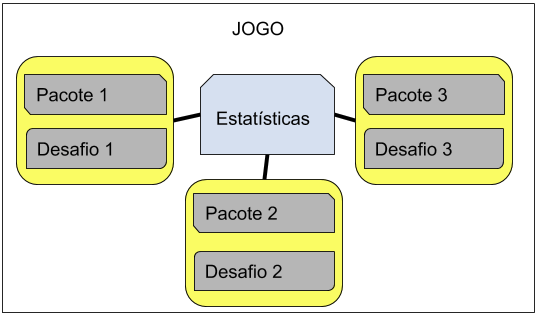
\includegraphics[scale=0.72]{figuras/pacote_jogo.png}
\label{pacoteDiagrama}
\small{Fonte: do próprio autor}
\end{figure}

\section[Pacote 1]{Pacote 1}
O pacote 1 trata a respeito de conhecimento de ED. Objetiva fixar o reconhecimento e classificação. Serão realizadas perguntas para que o jogador responda a respeito da ordem, tipo e linearidade das ED.

A fase 1 é a caminhada do estudante em uma estrada até o objetivo de Cálculo 3 (C3) e ele lidará com obstáculos no caminho. Para passar é preciso responder questões a respeito de classificação e reconhecimento da ED. Ao interagir com cada obstáculo ele será questionado sobre um exemplo de ED e terá que escolher 1 resposta entre 4 opções, sendo que nos níveis fáceis existem 2 respostas corretas a cada 4 opções. Com o evoluir da dificuldade o número de opções corretas cairá para 1. 

\begin{comment}
Solução geral e particular
\begin{itemize}
\item{ED ou não ED;}
\item{ED separável ou não;}
\item{ED homogênea ou não;}
\item{ED linear ou não linear;}
\item{ED exata ou não.}
\end{itemize}
\end{comment}

\begin{comment}
No desenvolvimento do jogo vamos usar exemplos de aplicações da EDO. Para controle de população, decaimento radioativo e juros no tempo. (entre outros exemplos a serem pensados)
O jogo terá tipos de fases e level. Os jogadores podem jogar o jogo de tempo de perguntas e respostas tanto de resposta de exercícios como resultados das situações no contexto real, que de preferência seja da vida do aluno e situações do dia-a-dia para ser mais próximo do ambiente de cada um.
O jogo abordará questões de definição e classificação das equações diferenciais.
\end{comment}

\section[Pacote 2]{Pacote 2}
O pacote 2 visa fixar o conhecimento de resolução de EDOs. Para isso jogaremos o jogo da memória.
Jogo da memória é para achar as cartas gêmeas. Uma carta contém o exercício proposto e a carta gêmea contém a resposta correta. Com o aumento do nível de dificuldade o jogo conterá mais pares e exercícios mais complexos. 


\section[Pacote 3]{Pacote 3}

O pacote três trata a respeito de aplicações de EDO.

\section[Estatísticas]{Estatísticas}
O módulo de estatísticas está relacionado à coleta de dados para a avaliação da quantidade de erros nas questões, quais foram as questões mais erradas e qual fase os estudantes tem mais dificuldade. O envio das estatísticas para o servidor não ocorrerá de forma programada, depende do jogador enviar os dados de acordo com a sua vontade de colaboração através de um botão pronto que esteja aguardando o envio das estatísticas.

\begin{comment}
No desafio do modo de jogo 1, o jogador corre contra o tempo para classificar o maior número de equações de possíveis. A cada 3 respostas consecutivas corretas serão adicionados 2 segundos de tempo. Ao fim do desafio ficará registrado o récorde de pontuação do jogador.

Na fase 2 que é o jogo da memória o jogador lidará com problemas de resolução de exercícios.
Uma carta é uma equação e a sua carta gêmea é a resposta da equação.
No início existem menos cartas e exercícios mais fáceis, conforme prossegue no nível de dificuldade aumentarão o número de cartas e a dificuldade dos exercícios.

No desafio do modo de jogo 2, é o jogo da memória ao inverso, todas as cartas mostram os seus valores   e ao clicar na carta ela vira de lado mostrando o desenho da estampa da carta. O objetivo a ser atingido é esconder o valor de todas as cartas sem cometer nenhum tropeço errando a combinação de pares. Ao fim do desafio ficará registrado a quantidade récorde do mínimo de tropeços do jogador.

No modo 3 o jogo será em terceira pessoa, o jogador estará imerso no labirinto ao invés de 2D (visão superior) igual o modo de jogo 1 e 2. Neste modo o jogador possui um avatar que pode se locomover pelo labirinto. O labirinto possui mais de uma maneira de chegar à saída, porém existem caminhos mais longos que outros. No labirinto os jogadores irão se deparar com problemas no caminho, onde precisarão resolver problemas de aplicações para poder passar. A vantagem do labirinto é que existe mais de um caminho para chegar ao fim e o jogador pode escolher outro caminho caso não esteja satisfeito com o primeiro escolhido. As questões de aplicação serão a respeito de crescimento de bactérias atrapalhando o caminho, trajetórias de projeteis lançados no jogador, escoamento de fluidos, transferência de calor para derretimento de barreiras.


Requisitos do jogo: \\
Responsivo; \\
\textit{Feedbacks} constantes ao fim de atividades com redirecionamento às próximas ações; \\
Instruções iniciais com pequenas etapas; \\
Complexidade das instruções devem ser progressivas; \\
Confirmação do objetivo esperado na atividade; \\
Variação das atividades para evitar cansaço; \\
Diversidade de itens para pessoa escolher o desejado.

\end{comment}

